\section{Modelo clásico}

\begin{figure}[t!]
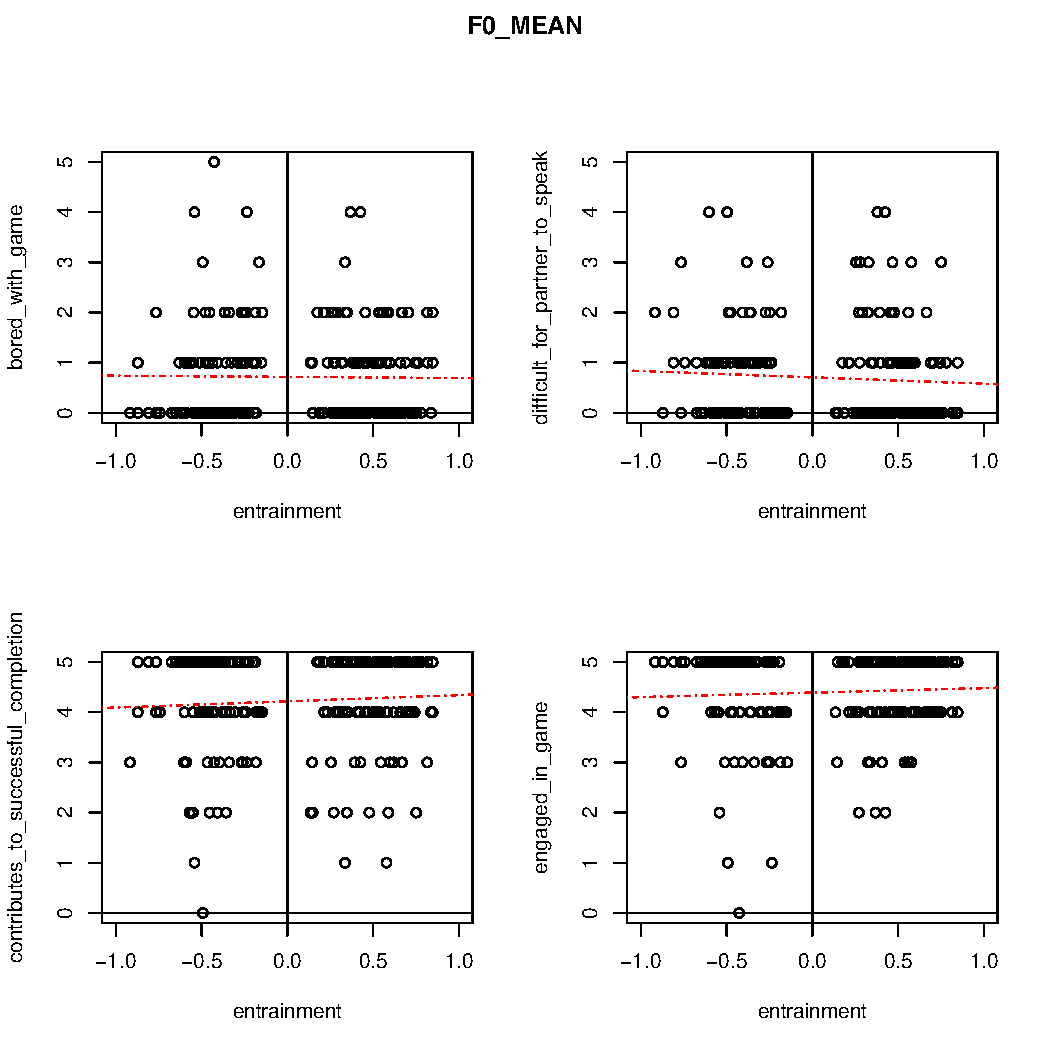
\includegraphics[width=15cm]{images/regression_F0_MEAN_1.pdf}
\caption{Gráfico de los pares entrainment-variable a/p, junto a la regresión lineal obtenida \label{regresion_clasica} para \emph{F0\_MEAN}}
\end{figure}

En el modelo clásico no dio resultados apreciables, principalmente por la baja significancia de sus resultados. En \ref{regresion_clasica} puede verse el gráfico de \emph{F0\_MEAN} y 4 variables sociales y en \ref{regresion_clasica_tabla} pueden verse los valores de las estimaciones de $\widehat{\beta_2}$ junto a sus p-valores.


\begin{figure}[l]
% "ENG_MEAN"
% latex table generated in R 3.2.2 by xtable 1.8-0 package
% Thu Jan  7 03:01:56 2016
\begin{tabular}{rrrrr}
  \hline
 ENG\_MEAN & $\widehat{\beta_2}$ & Std. Error & t value & Pr($>$$|$t$|$) \\
  \hline
  bored\_with\_game & 10.6496 & -0 & 2.036037E-21 & 0.6587 \\
  difficult\_for\_partner\_to\_speak & 10.5625 & -1 & 3.728189E-21 & 0.5893 \\
  contributes\_to\_successful\_completion & 59.6193 & -1 & 9.639522E-133 & 0.2519 \\
  engaged\_in\_game & 73.1439 & 1 & 2.276897E-150 & 0.5851 \\
  gives\_encouragement & 47.4920 & -0 & 1.314327E-113 & 0.9659 \\
  making\_self\_clear & 52.9691 & -1 & 1.022216E-122 & 0.3253 \\
  planning\_what\_to\_say & 32.0193 & -2 & 2.465471E-82 & 0.0718 \\
  dislikes\_partner & 9.6126 & -1 & 2.462398E-18 & 0.3482 \\  \hline
\end{tabular}

% latex table generated in R 3.2.2 by xtable 1.8-0 package
% Fri Jan  8 00:50:24 2016
\begin{tabular}{rrrrr}
  \hline
 ENG\_MAX & $\widehat{\beta_2}$ & Std. Error & t value & Pr($>$$|$t$|$) \\
  \hline
bored\_with\_game & 10.4714 & 0 & 7.003232E-21 & 0.9053 \\
  difficult\_for\_partner\_to\_speak & 10.3984 & -0 & 1.160098E-20 & 0.9678 \\
  contributes\_to\_successful\_completion & 58.9660 & -0 & 8.397021E-132 & 0.6739 \\
  engaged\_in\_game & 72.6730 & 1 & 8.299021E-150 & 0.6008 \\
  gives\_encouragement & 47.3103 & -0 & 2.727411E-113 & 0.6494 \\
  making\_self\_clear & 52.2454 & 1 & 1.465061E-121 & 0.3220 \\
  planning\_what\_to\_say & 31.1729 & 0 & 2.491793E-80 & 0.7176 \\
  dislikes\_partner & 9.5924 & -1 & 2.820254E-18 & 0.3279 \\
   \hline
\end{tabular}

% latex table generated in R 3.2.2 by xtable 1.8-0 package
% Thu Jan  7 03:01:56 2016
\begin{tabular}{rrrrr}
  \hline
F0\_MEAN & $\widehat{\beta_2}$ & Std. Error & t value & Pr($>$$|$t$|$) \\
  \hline
bored\_with\_game & 10.6286 & -0 & 2.355933E-21 & 0.8572 \\
  difficult\_for\_partner\_to\_speak & 10.6764 & -1 & 1.689495E-21 & 0.3316 \\
  contributes\_to\_successful\_completion & 59.3792 & 1 & 2.130619E-132 & 0.3726 \\
  engaged\_in\_game & 73.4118 & 1 & 1.094910E-150 & 0.4425 \\
  gives\_encouragement & 47.5948 & 1 & 8.705216E-114 & 0.2774 \\
  making\_self\_clear & 52.9055 & -0 & 1.290163E-122 & 0.7471 \\
  planning\_what\_to\_say & 31.4874 & 0 & 4.441831E-81 & 0.6977 \\
  dislikes\_partner & 9.8092 & -2 & 6.530815E-19 & 0.0835 \\
   \hline
\end{tabular}

% ""
% latex table generated in R 3.2.2 by xtable 1.8-0 package
% Thu Jan  7 03:01:56 2016
\begin{tabular}{rrrrr}
  \hline
F0\_MAX & $\widehat{\beta_2}$ & Std. Error & t value & Pr($>$$|$t$|$) \\
  \hline
bored\_with\_game & 11.0806 & 2 & 1.001502E-22 & 0.0147 \\
  difficult\_for\_partner\_to\_speak & 10.6511 & 1 & 2.014306E-21 & 0.6023 \\
  contributes\_to\_successful\_completion & 60.0792 & -1 & 2.127331E-133 & 0.3297 \\
  engaged\_in\_game & 74.2016 & -1 & 1.282700E-151 & 0.5711 \\
  gives\_encouragement & 48.1664 & -1 & 8.925956E-115 & 0.2986 \\
  making\_self\_clear & 53.8649 & -2 & 3.954497E-124 & 0.0212 \\
  planning\_what\_to\_say & 31.8577 & -1 & 5.915312E-82 & 0.2950 \\
  dislikes\_partner & 9.6545 & 1 & 1.857261E-18 & 0.3340 \\
  \hline
\end{tabular}


\caption{Tablas con los resultados de la regresión clásica para ENG\_MEAN, ENG\_MAX, F0\_MEAN y F0\_MAX. En la segunda columna se cita el valor de $\widehat{\beta_2}$, la desviación estándar calculada, el t-valor obtenido y la significancia}\label{regresion_clasica_tabla}
\end{figure}

